\subsection{BÀI TẬP TRẮC NGHIỆM}
\ind{PHẦN I.} \inden{Câu trắc nghiệm nhiều phương án lựa chọn. Mỗi câu hỏi học sinh chỉ chọn một phương án.}\\
\setcounter{ex}{0}
\Opensolutionfile{ans}[ans/1D6-B3-1]
\begin{ex}
	(THPTQG 2021 -- Mã đề 101). Tập xác định của hàm số $y=9^x$
	\choice
	{\True $\mathbb R$}
	{$[0;+\infty)$}
	{$\mathbb R\setminus\{0\}$}
	{$(0;+\infty)$}
	\loigiai{
		Cần chú ý lý thuyết: Với $a>$ và $a \ne 1$
		\begin{itemize}
			\item [$\bullet$] Hàm số $y=a^x$ có tập xác định là $\mathbb{R}$
			\item [$\bullet$]  Hàm số $y=a^x$ có tập giá trị là $(0;+\infty)$ (Đồ thị luôn trên trục $Ox$).
		\end{itemize}
	}
\end{ex}
\begin{ex}
	Tập xác định của hàm số $y=\log_3{x}$ là
	\choice
	{$\left[0;+\infty \right)$}
	{$\mathbb{R}\setminus {\left\lbrace 0\right\rbrace}$}
	{$\mathbb{R}$}
	{\True $\left(0;+\infty \right)$}
	\loigiai{
		Hàm số $y=\log_3{x}$ xác định trên $\left(0;+\infty \right)$.
	}
\end{ex}

\begin{ex}
	Hàm số nào trong các hàm số sau đây có tập xác định là $\mathbb R$?
	\choice
	{$y=\log_2x$}
	{$y=\dfrac{2x-1}{x+1}$}
	{$y=\tan x$}
	{\True $y=x^3-3x^2+4x-1$}
	\loigiai{
		\begin{itemize}
			\item Hàm $y=\log_2x$ có $\mathscr{D}=(0;+\infty)$.
			\item Hàm $y=\dfrac{2x-1}{x+1}$ có $\mathscr{D}=\mathbb R\setminus\{-1\}$.
			\item Hàm $y=\tan x$ có $\mathscr{D}=\mathbb R\setminus\left\{\dfrac{\pi}{2}+k\pi|k\in\mathbb Z\right\}$.
			\item Hàm $y=x^3-3x^2+4x-1$ có $\mathscr{D}=\mathbb R$.
		\end{itemize}
	}
\end{ex}

\begin{ex}
	Tập xác định $ \mathscr{D} $ của hàm số $ y= \log_{2018} (2x - 1) $ là
	\choice
	{$ \mathscr{D} = (0;+\infty) $}
	{$ \mathscr{D} = \mathbb{R} $}
	{\True $ \mathscr{D} = \left (\dfrac{1}{2};+\infty \right )   $}
	{$ \mathscr{D} = \left [ \dfrac{1}{2};+\infty \right ) $}
	\loigiai{
		Hàm số xác định $ \Leftrightarrow 2x-1> 0 \Leftrightarrow x > \dfrac{1}{2} $.
	}	
\end{ex}

\begin{ex}
	Tìm tập xác định $D$ của hàm số y = $\log_2\sqrt{6-x}.$
	\choice
	{$D=\mathbb{R}\backslash \left\{6\right\}$}
	{$D=\left(-\infty; 6\right)$}
	{\True $D=\left(6;+\infty \right)$}
	{$D=\left(-\infty;6\right]$}
	\loigiai{
		Hàm số xác định khi và chỉ khi: $6-x>0 \Leftrightarrow x <6$.\\
		Vậy tập xác định của hàm số là $\mathscr{D}=\left( - \infty; 6 \right)$.
	}
\end{ex}

\begin{ex}
	Tập xác định của hàm số $y=\ln |4-x^2|$ là
	\choice
	{  $\mathbb{R}\backslash [-2;2]$ }
	{\True $\mathbb{R}\backslash \{-2;2\}$  }
	{ $\mathbb{R}$ }
	{$(-2;2)$  }
	\loigiai{
		Điều kiện: $4-x^2\ne 0\Leftrightarrow x\ne -2\: \text{và}\: x\ne 2$.
	}
\end{ex}

\begin{ex}
	Hàm số $y=\log_5 (4x-x^2)$ có tập xác định là 
	\choice
	{$\mathscr{D}=(0;+\infty)$}
	{\True $\mathscr{D}=(0;4)$}
	{$\mathscr{D}=\mathbb{R}$}
	{$\mathscr{D}=(-\infty;0)\cup (4;+\infty)$} 
	\loigiai{
		Hàm số xác định khi và chỉ khi $4x-x^2>0 \Leftrightarrow 0<x<4$.\\
		Vậy tập xác định $\mathscr{D}=(0;4)$.
	}
\end{ex}

\begin{ex}
	Tìm tập xác định $\mathscr{D}$ của hàm số $y=\log(x^2+2x+3)$.
	\choice
	{$\mathscr{D}=\mathbb{R}\setminus \{-2;-1\}$}
	{\True $\mathscr{D}=\mathbb{R}$}
	{$\mathscr{D}=\varnothing$}
	{$ \mathscr{D}=(-\infty ;-2) \cup (-1;+\infty)$}
	\loigiai{
		Điều kiện xác định của hàm số là $x^2+2x+3>0$ (đúng $\forall x \in \mathbb{R}$).}
\end{ex}

\begin{ex}
	Tập xác định của hàm số $y=\dfrac{\sqrt{x+1}}{\ln(5-x)}$ là
	\choice
	{$\mathbb{R}\setminus\{4\}$}
	{\True $[-1;5)\setminus\{4\} $}
	{$(-1;5)$}
	{$[-1;5]$}
	\loigiai{
		Hàm số xác định khi $\heva{&x+1\ge 0\\&5-x>0\\&\ln(5-x)\neq 0}\Leftrightarrow \heva{&x\ge -1\\&x<5\\&5-x\neq 1}\Leftrightarrow \heva{&-1\le x < 5\\&x\neq 4.}$\\  Vậy tập xác định là  $\mathscr{D}=[-1;5)\setminus\{4\}$.
	}
\end{ex}

\begin{ex}
	Hàm số nào trong các hàm số sau đây nghịch biến trên $\mathbb{R}$?
	\choice
	{$y=9^x$}
	{$y=\log_{0{,}9}x$}
	{$y=\log_9x$}
	{\True $y=\left(0{,}9\right)^x$}
	\loigiai{
		Trong các hàm số đã cho, hàm số $y=\left(0{,}9\right)^x$ là hàm số nghịch biến trên $\mathbb{R}$.
	}
\end{ex}

\begin{ex}%[1D4Y3-3]
	Tìm tất cả các giá trị của $a$ thỏa mãn $(a-1)^{-\dfrac{2}{3}}<(a-1)^{-\dfrac{1}{3}}$.
	\choice{$0<a<1$}{$a>1$}{$1<a<2$}{\True$a>2$}
	\loigiai{
		Ta có $(a-1)^{-\dfrac{2}{3}}<(a-1)^{-\dfrac{1}{3}}$ và $-\dfrac{2}{3}<-\dfrac{1}{3}$ nên $a-1> 1 \Leftrightarrow a >2$.
	}
\end{ex}

\begin{ex}%[2D2Y4-3]
	Hàm số nào sau đây đồng biến trên $\mathbb{R}$?
	\choice
	{$y=\left( \dfrac{3}{\pi} \right)^x$}
	{\True $y=\left( \dfrac{\sqrt{2}+\sqrt{3}}{\mathrm{e}} \right)^x$}
	{$y=\log_7 \left( x^4+5 \right)$}
	{$y=\left(\dfrac{\sqrt{2018}-\sqrt{2015}}{10^{-1}}\right)^x$}
	\loigiai{
		Ta có $\dfrac{\sqrt{2}+\sqrt{3}}{\mathrm{e}}>1$ nên hàm số $y=\left( \dfrac{\sqrt{2}+\sqrt{3}}{\mathrm{e}} \right)^x$ đồng biến trên $\mathbb{R}$.
	}
\end{ex}

\begin{ex}
	Cho các số thực $a,~b$ thỏa mãn $0<a<1<b$. Khẳng định nào sau đây đúng?
	\choice
	{\True $\log_a b<0$}
	{$(0{,}5)^a<(0{,}5)^b$}
	{$\ln a>\ln b$}
	{$2^a>2^b$}
	\loigiai
	{
		Theo giả thiết đề bài thì
		\begin{itemize}
			\item Hàm số $y=\log_a x$ nghịch biến trên $(0;+\infty)$ nên $b>1\Rightarrow\log_a b<\log_a1=0$.
			\item Hàm số $y=\ln x$ đồng biến trên $(0;+\infty)$ nên $a<b\Rightarrow\ln a <\ln b$.
			\item Hàm số $y=0{,5}^x$ nghịch biến trên $\mathbb{R}$ nên $a<b\Rightarrow(0{,}5)^a>(0{,}5)^b$.
			\item Hàm số $y=2^x$ đồng biến nên trên $\mathbb{R}$ $a<b\Rightarrow 2^a<2^b$.
		\end{itemize}
		Vậy khẳng định đúng là $\log_a b<0$.
	}
\end{ex}

\begin{ex}
	Trong các mệnh đề sau, mệnh đề nào là mệnh đề {\bf sai}?
	\choice
	{Nếu $0<a<b$ thì $\ln a<\ln b$}
	{\True Nếu $0<a<b$ thì $\log_{\tfrac{\pi}{4}} a<\log_{\tfrac{\pi}{4}}b$}
	{Nếu $0<a<b$ thì $\log_{\tfrac{\mathrm{e}}{2}} a<\log_{\tfrac{\mathrm{e}}{2}} b$}
	{Nếu $0<a<b$ thì $\log a<\log b$}
	\loigiai{
		Vì $\dfrac{\pi}{4}<1$ nên hàm số $y= \log_{\tfrac{\pi}{4}} x$ nghịch biến trên khoảng $(0; +\infty)$.\\
		$\Rightarrow$ Mệnh đề \,\lq\lq Nếu $0<a<b$ thì $\log_{\tfrac{\pi}{4}} a<\log_{\tfrac{\pi}{4}}b$\rq\rq\, là mệnh đề sai.
	}
\end{ex}


\begin{ex}
	Tìm tất cả các giá trị của $a$ để hàm số $y = (2020 - a)^x$ nghịch biến trên $\mathbb{R}$.
	\choice
	{$ a<2019$}
	{$ a<2020 $}
	{\True $2019 < a < 2020 $}
	{$ 0<a<1 $}
	\loigiai{
		Để hàm số $y = (2020 - a)^x$ nghịch biến trên $\mathbb{R}$ thì $0 < 2020 - a < 1 \Leftrightarrow 2019 < a < 2020$.
	}
\end{ex}

\begin{ex}
	\immini[thm]{
		Đồ thị sau đây là của hàm số nào?
		\haicot
		{\True $y=2^x$}
		{$y=\log_{\dfrac{1}{2}}x$}
		{$y={\left(\dfrac{1}{2}\right)}^x$}
		{$y=\log_2x$}
	}{
		\begin{tikzpicture}[scale=0.6,>=stealth,x=1cm,
			y=1cm]
			\def \xmin{-2.5}
			\def \xmax{3.5}
			\def \ymin{-0.66}
			\def \ymax{3.98}
			% Vẽ 2 trục, điền các số lên trục
			\draw[->] (\xmin,0) -- (\xmax,0);
			\draw[->,color=black] (0,\ymin) -- (0,\ymax);
			\draw[color=black](\xmax-0.3,.2)node[right] {$x$};
			\draw[color=black] (.1,\ymax) node[right] {\normalsize $y$};
			\draw[color=black] (0pt,-8pt) node[left] {\normalsize $O$};
			\begin{scope}
				\clip(\xmin ,\ymin) rectangle (\xmax-1,\ymax-0.5);
				%Vẽ đồ thị
				\draw[smooth,samples=100,domain=\xmin:\xmax] 
				plot(\x,{2^(\x)});
			\end{scope}
			\node at (-.3,1.3){1};
		\end{tikzpicture} 
	}
	\loigiai{
		Hàm số đồng biến trên $\mathbb{R}$ nên loại các phương án $y=\left( \dfrac{1}{2} \right)^x, \; y=\log_{\dfrac{1}{2}}x$ và $y=\log_2 x$.
	}
\end{ex}

\begin{ex}%[2D2Y4-3]%
	\immini[thm]{Đồ thị có trong hình vẽ kề bên là của hàm số nào dưới đây?
		\haicot
		{\True $y={\left(\dfrac{1}{3} \right)}^x$}
		{$y={(\sqrt{2})}^x$}
		{$y={(\sqrt{3})}^x$}
		{$y={\left(\dfrac{1}{2} \right)}^x$}
	}
	{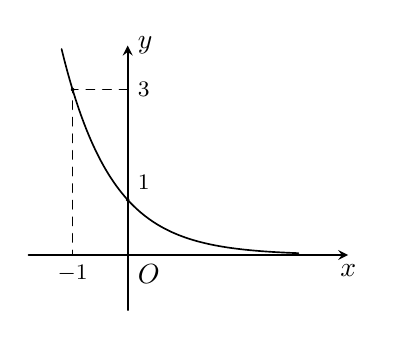
\begin{tikzpicture}[line width=0.6pt,line cap=round,line join=round,>=stealth,smooth,samples=300,scale=0.7]
			\draw[->] (-1.8,0)--(4,0) node[below]{$x$};
			\draw[->] (0,-1)--(0,3.8) node[right]{$y$};
			\node at (0,0) [below right]{$O$};
			\draw[domain=-1.2:3.1] plot(\x,{(1/3)^(\x)});
			\draw[dashed] (0,3)--(-1,3)--(-1,0);
			\node at (0,3) [right]{\footnotesize $3$};
			\node at (-1,0) [below]{\footnotesize $-1$};
			\draw (0,1) circle(0.6pt) node [above right]{\footnotesize $1$};
			\draw (-1,3) circle(0.6pt);
	\end{tikzpicture}}
	\loigiai{
		Đồ thị hàm số trong hình chỉ có thể là của hàm số nghịch biến trên $\mathbb{R}$ nên hàm số $y=(\sqrt{3})^x$ và $y=(\sqrt{2})^x$ bị loại.\\
		Ngoài ra do đồ thị hàm số đi qua điểm $A(-1;3)$ nên chỉ còn hàm số $y={\left(\dfrac{1}{3} \right)}^x$ thoả mãn.}
\end{ex}

\begin{ex}
	\immini[thm]{
		Đồ thị hàm số như hình vẽ bên là đồ thị của hàm số nào?
		\haicot
		{\True $y=\log_{\tfrac{1}{2}}x$}
		{$y=2^{x}$}
		{$y=\log_{2}x$}
		{$y=\left(\dfrac{1}{2}\right)^{x}$}
	}{
		\begin{tikzpicture}[>=stealth,yscale=0.7]
			\tikzset{label style/.style={font=\footnotesize}}
			\def\hsloganb{ln(\x)/ln(1/2)}
			\def\xmax{4}
			\def\xmin{-1}
			\def\ymax{2.5}
			\def\ymin{-1.5}
			\begin{scope}
				\clip (\xmin,\ymin) rectangle (\xmax,\ymax);
				\draw[-stealth] (\xmin,0)--(\xmax,0) node[below left]{$x$};
				\draw[-stealth] (0,\ymin)--(0,\ymax) node[below left]{$y$};
				\draw[samples=100,domain=0.1:\xmax,smooth,variable=\x]plot(\x,{\hsloganb});
				\draw(0,0)node[below right]{\fontsize{12pt}{1pt}\selectfont $O$};
				\path (1,0) node[below]{$1$};
			\end{scope}
		\end{tikzpicture}
	}
	\loigiai{
		Dựa vào đồ thị ta thấy hàm số nghịch biến, suy ra cơ số của hàm mũ (hoặc logarit) phải nhỏ hơn $1$. Lại có đồ thị hàm số đi qua điểm $(1;0)$nên đây là đồ thị của hàm số $y=\log_{\tfrac{1}{2}}x$.
	}
\end{ex}

\begin{ex}
	\immini[thm]{Cho $a, b, c$ là các số thực dương, khác 1. Đồ thị các hàm số $y=a^x, y=b^x, y=c^x$ được cho trong hình vẽ dưới đây. Mệnh đề nào sau đây đúng?
		\choice
		{$1<a<c<b$}
		{\True $a<1<c<b$}
		{$a<1<b<c$}
		{$1<a<b<c$}}
	{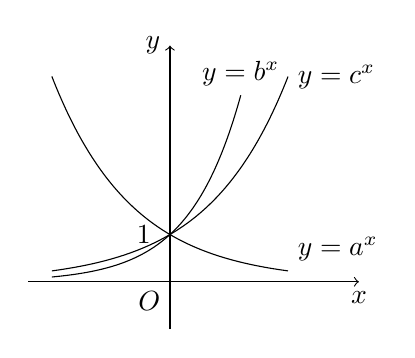
\begin{tikzpicture}[scale=0.6]
			\draw[->] (-3,0)--(0,0) node[below left]{$O$}--(4,0) node[below] {$x$};
			\draw[->] (0,-1)-- (0,5) node[left]{$y$};
			\node[left] at (-.2,1) {$1$};
			\draw[smooth,samples=100,domain=-2.5:2.5] plot(\x,{1/(1.8^(\x))}) node[above right]{$y=a^x$};
			\draw[smooth,samples=100,domain=-2.5:1.5] plot(\x,{2.5^(\x)}) node[above]{$y=b^x$};
			\draw[smooth,samples=100,domain=-2.5:2.5] plot(\x,{1.8^(\x)}) node[right]{$y=c^x$};
	\end{tikzpicture}}
	\loigiai{\immini{Xét đường thẳng $x=1$. Nó cắt các đường cong $y=a^x, y=b^x, y=c^x, y=1$ lần lượt tại các điểm mà tung độ là $a, b, c, 1$. Căn cứ vào đồ thị đã cho, ta suy ra $a<1<c<b.$}
		{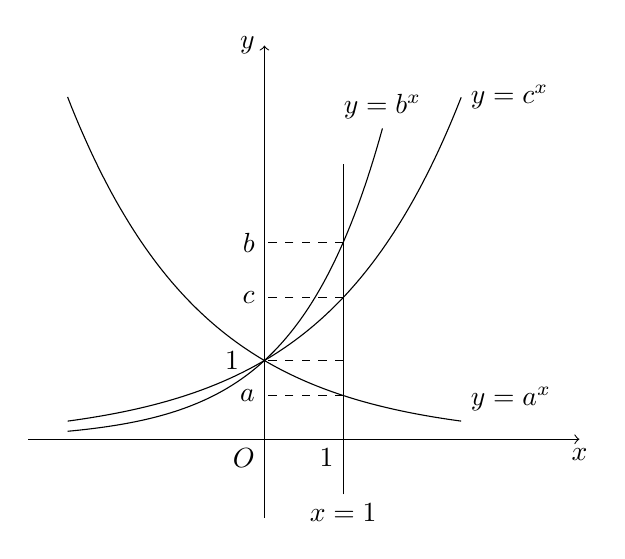
\begin{tikzpicture}
				\draw[->] (-3,0)--(0,0) node[below left]{$O$}--(4,0) node[below] {$x$};
				\draw[->] (0,-1)-- (0,5) node[left]{$y$};
				\node[left] at (-.2,1) {$1$};
				\draw[-](1,-.7) node[below]{$x=1$}--(1,0) node[below left]{$1$}--(1,3.5);
				\draw[-][dashed](1,.5556)--(0,.5556) node[left]{$a$};
				\draw[-][dashed](1,1.8)--(0,1.8) node[left]{$c$};
				\draw[-][dashed](1,2.5)--(0,2.5) node[left]{$b$};
				\draw[-][dashed](1,1)--(0,1);
				\draw[smooth,samples=100,domain=-2.5:2.5] plot(\x,{1/(1.8^(\x))}) node[above right]{$y=a^x$};
				\draw[smooth,samples=100,domain=-2.5:1.5] plot(\x,{2.5^(\x)}) node[above]{$y=b^x$};
				\draw[smooth,samples=100,domain=-2.5:2.5] plot(\x,{1.8^(\x)}) node[right]{$y=c^x$};
			\end{tikzpicture}
		}
	}
\end{ex}

\begin{ex}
	\immini[thm]{
		Cho $a,b,c$ là các số thực dương khác $1$.  Hình vẽ bên là đồ thị của hàm số $y=\log_x$, $y=\log_b x$, $y=\log_c x$. Khẳng định nào sau đây đúng?
		\choice
		{$a<b<c$}
		{\True $b<c<a$}
		{$b<a<c$}
		{$c<a<b$}
	}
	{
		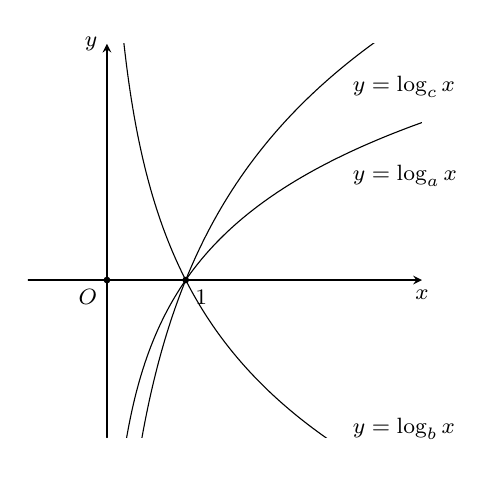
\begin{tikzpicture}[scale=1, font=\footnotesize, line join=round, line cap=round, >=stealth]
			\draw[->] (-1,0)--(4,0) node[below] {$x$};
			\draw[->] (0,-2)--(0,3) node[left] {$y$};
			\draw[fill=black] (0,0) circle(1pt) node[below left] {$O$};
			\draw[fill=black] (1,0) circle(1pt) node[below right] {$1$};
			\draw (3,1.58) node[below right]  {$y=\log_a x$};
			\draw (3,-2.15) node[above right]  {$y=\log_b x$};
			\draw (3,2.71) node[below right]  {$y=\log_c x$};
			\clip (0,-2) rectangle (4,3) ;
			\draw[samples=100,smooth,domain=0.1:4] plot(\x,{ln(\x)/ln(0.6)});
			\draw[samples=100,smooth,domain=0.1:4] plot(\x,{ln(\x)/ln(2)});
			\draw[samples=100,smooth,domain=0.1:4] plot(\x,{ln(\x)/ln(1.5)});
		\end{tikzpicture}
	}
	\loigiai{
		Từ đồ thị hàm số suy ra $b<1<c<a$.
	}
\end{ex}

\begin{ex}
	\immini[thm]{Cho ba hàm số $ y=a^x, y=b^x, y=\log_cx $ lần lượt có đồ thị $ (C_1),(C_2), (C_3) $ như hình bên. Mệnh đề nào sau đây đúng?
		\haicot
		{\True $ a>b>c $}
		{$ b>a>c $}
		{$ c>b>a $}
		{$ c>a>b $}}
	{   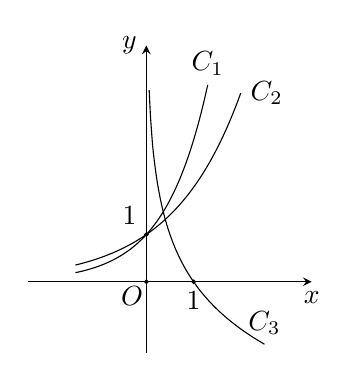
\begin{tikzpicture}[scale=0.6,>=stealth]
			\draw[->](0,-1.5)--(0,5) node [left] {$y$};
			\draw[->](-2.5,0)--(3.5,0) node [below] {$x$};
			%\clip (-1.5,5)rectangle (3.5,-3);
			\draw[smooth,samples=100,domain=-1.5:2] plot({\x},{(2)^(\x)}) node[right]{$ C_2 $};
			\draw[smooth,samples=100,domain=-1.5:1.3] plot({\x},{(3)^(\x)}) node[above]{$ C_1 $};
			\draw[smooth,samples=100,domain=.06:2.5] plot(\x,{ln(\x)/ln(1/2)})node[above] {$C_3$}; 	
			\node at (-0.3,-0.3) {$O$};
			\node[above left] at (0,1) {$1$};
			\node[below] at (1,0) {$1$};
			\draw[fill=black] (0,1) circle (1pt);
			\draw[fill=black] (1,0) circle (1pt);  
			\draw[fill=black] (0,0) circle (1pt);  
		\end{tikzpicture}
	}
	\loigiai{
		Quan sát trên đồ thị ta thấy đồ thị hàm số $ y=a^x, y=b^x $ đồng biến trên $ \mathbb{R} $ nên $ a>1,b>1 .
		\\
		$ Với $ x=1\Rightarrow a^1>b^1 $ hay $ a>b $.\\
		Quan sát đồ thị $ \left(C_3\right )  $ nghịch biến $ \Rightarrow c<1. $\\
		Vậy $ a>b>c. $
	}
\end{ex}


\begin{ex}
	\immini[thm]{
		Cho hàm số $y = \log_{a}x$ và $y = \log_{b}x$ có đồ thị lần lượt là $\left(C\right)$ và $\left(C'\right)$ (như hình vẽ bên). Đường thẳng $x = 9$ cắt trục hoành và các đồ thị $\left(C\right)$ và $\left(C'\right)$ lần lượt tại $M$, $N$ và $P$. Biết rằng $MN = NP$, hãy xác định biểu thức liên hệ giữa $a$ và $b$
		\haicot
		{\True $a = b^{2}$}
		{$a = 9b$}
		{$a = 3b$}
		{$a = b + 3$}
	}{\hspace{1cm}
		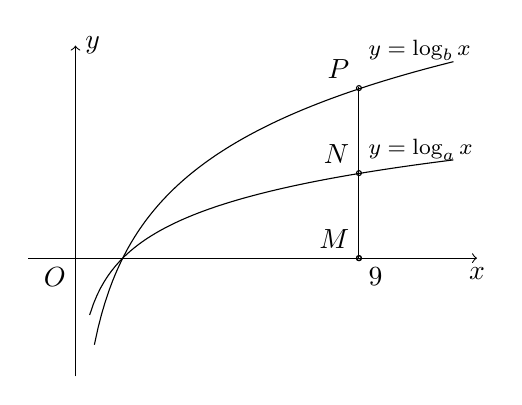
\begin{tikzpicture}[scale=0.6]	
			%\clip(-1, -1) rectangle (8, 8);
			\draw[->] (-1,0) --(0,0) node[below left]{$O$}--(8.5,0) node[below]{$x$};
			\draw[->] (0,-2.5) --(0,4.5) node[right]{$y$};
			\draw (6,0) node[below right]{$9$} circle (1.5pt);
			\draw (6,0) node[above left]{$M$} circle (1.5pt);
			\draw (6,1.8) node[above left]{$N$} circle (1.5pt);
			\draw (6,3.6) node[above left]{$P$} circle (1.5pt);
			\draw [samples=100, domain=0.3:8] plot (\x, {(ln(\x))}) (6,2.3) node[right]{\footnotesize $y = \log_{a}x$};
			\draw [samples=100, domain=0.4:8] plot (\x, {2*(ln(\x))}) (6,4.4) node[right]{\footnotesize $y = \log_{b}x$};
			\draw [-] (6,0)--(6,3.63);
		\end{tikzpicture}
	}
	\loigiai{Dựa vào đồ thị suy $a > b$ và $N$ thuộc đồ thị  
		$y = \log_{a}x$ và $P$ thuộc đồ thị hàm số $y = \log_{b}x$. Do giả thiết suy ra $MN = \log_{a}9$ và 
		$MP = \log_{b}9$. Vì $MN = NP$ suy ra $MP = 2MN$ nên 
		$$\log_{b}9 = 2\log_{a}9\Leftrightarrow \dfrac{1}{\log_{9}b} = \dfrac{2}{\log_{9}a}\Leftrightarrow \log_{9}a = 2\log_{9}b\Leftrightarrow \log_{9}a = \log_{9}b^2\Leftrightarrow a = b^2.$$  	
	}
\end{ex}

\begin{ex}
	\immini[thm]{Trong hình vẽ bên các đường cong $\left(C_{1}\right)\colon y=a^{x}$, $\left(C_{2}\right)\colon y=b^{x}$, $\left(C_{3}\right)\colon y=c^{x}$ và đường thẳng	$y=4$ cắt các đường cong $\left(C_{1}\right)$, $\left(C_{2}\right)$, $\left(C_{3}\right)$ lần lượt tại các điểm $A$, $ B$, $C$, $D$ sao cho $H A=A B=B C$. Khẳng định nào sau đây là đúng?
		\choice
		{$ac^2=b^3$}
		{$a+3c=4b$}
		{\True $ac^3=b^4$}
		{$a+2c=3b$}
	}
	{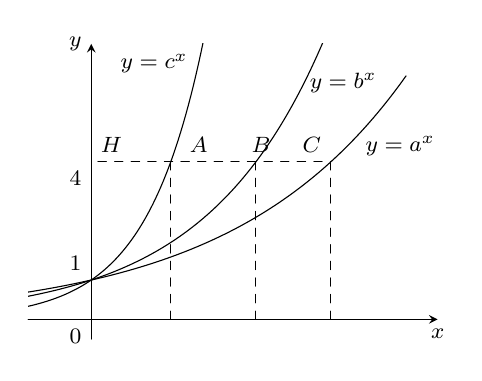
\begin{tikzpicture}[scale=1, font=\footnotesize, line join=round, line cap=round, >=stealth,yscale=0.5,xscale=0.8]
			\tkzInit[xmin = -3,xmax = 5.5,ymin =-0.5,ymax =7]
			\draw [->](-1,0) -- (5.5,0) node[below]{$x$}; \draw [->](0,-0.5) -- (0,7) node[left]{$y$};
			%\draw[-] (-3,4)--(5.5,4);
			\node[below left] at (0,0) {$0$};
			\clip(-1,-0.5) rectangle (5.5,7);
			\draw[ domain=-3:5,samples=200] plot (\x, {3^(\x)});
			\draw[domain=-3:5,samples=200] plot (\x, {1.7^(\x)});
			\draw[domain=-3:5,samples=200] plot (\x, {1.44^(\x)});
			\node[above left] at (0,1) {\footnotesize $1$}; \node[] at (4,6) {\footnotesize $y=b^x$};\node[] at (1,6.5) {\footnotesize $y=c^x$};
			\node[above right] at (0,4) {\footnotesize $H$}; \node[below left] at (0,4) {\footnotesize $4$};
			\node[above left] at (2,4) {\footnotesize $A$}; \node[above left] at (3,4) {\footnotesize $B$};\node[above left] at (3.80178401692,4) {\footnotesize $C$};\node[right] at (4.2,4.4) {\footnotesize $y=a^x$};
			\draw [dashed](1.26185950714,0)--(1.26185950714,4);
			\draw [dashed](2.6125528717,0)--(2.6125528717,4);
			\draw [dashed](3.80178401692,0)--(3.80178401692,4)--(0,4);
	\end{tikzpicture}}
	\loigiai{
		\immini{$H A=A B=B C \Rightarrow x_3=3 x_1$ và $x_2=2 x_1$ với $x_1$, $x_2$, $x_3$ lần lượt là hoành độ của các điểm $A$, $B$, $C$.\\
			$\Rightarrow c^{x_1}=\left(b^{x_1}\right)^2=\left(a^{x_1}\right)^3=4 \Rightarrow\left(a c^3\right)^{x_1}=\left(b^4\right)^{x_1} \Rightarrow a c^3=b^4$.}
		{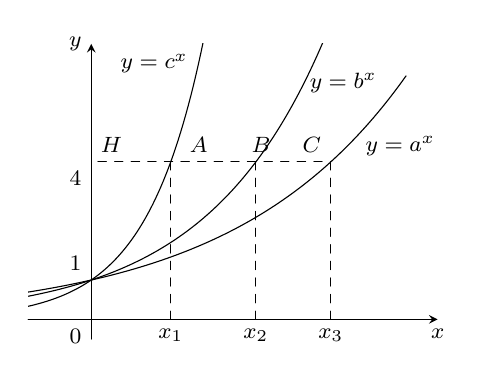
\begin{tikzpicture}[scale=1, font=\footnotesize, line join=round, line cap=round, >=stealth,yscale=0.5,xscale=0.8]
				\tkzInit[xmin = -3,xmax = 5.5,ymin =-0.5,ymax =7]
				\draw [->](-1,0) -- (5.5,0) node[below]{$x$}; \draw [->](0,-0.5) -- (0,7) node[left]{$y$};
				%\draw[-] (-3,4)--(5.5,4);
				\node[below left] at (0,0) {$0$};
				\clip(-1,-1) rectangle (5.5,7);
				\draw[ domain=-3:5,samples=200] plot (\x, {3^(\x)});
				\draw[domain=-3:5,samples=200] plot (\x, {1.7^(\x)});
				\draw[domain=-3:5,samples=200] plot (\x, {1.44^(\x)});
				\node[above left] at (0,1) {\footnotesize $1$}; \node[] at (4,6) {\footnotesize $y=b^x$};\node[] at (1,6.5) {\footnotesize $y=c^x$};
				\node[above right] at (0,4) {\footnotesize $H$}; \node[below left] at (0,4) {\footnotesize $4$};
				\node[above left] at (2,4) {\footnotesize $A$}; \node[above left] at (3,4) {\footnotesize $B$};\node[above left] at (3.80178401692,4) {\footnotesize $C$};\node[right] at (4.2,4.4) {\footnotesize $y=a^x$};\node[below] at (1.26185950714,0) {\footnotesize $x_1$}; \node[below] at (2.6125528717,0) {\footnotesize $x_2$}; \node[below] at (3.80178401692,0) {\footnotesize $x_3$};
				\draw [dashed](1.26185950714,0)--(1.26185950714,4);
				\draw [dashed](2.6125528717,0)--(2.6125528717,4);
				\draw [dashed](3.80178401692,0)--(3.80178401692,4)--(0,4);
		\end{tikzpicture}}
	}
\end{ex}


\begin{ex}%[2D2G4-3]
	Đồ thị hàm số $y=f(x)$ đối xứng với đồ thị của hàm số $y=a^x$ $(a>0,a\neq 1)$ qua điểm $(1;1)$. Giá trị của biểu thức $f\left(2+\log_a\dfrac{1}{2018}\right)$ bằng
	\choice
	{\True $-2016$}
	{$-2020$}
	{$2016$}
	{$2020$}
	\loigiai{
		Xét $M\left(2+\log_a\dfrac{1}{2018};f\left(2+\log_a\dfrac{1}{2018}\right)\right)$ thuộc đồ thị hàm số $ y=f(x)$.\\
		Điểm $N\left(-\log_a\dfrac{1}{2018};2-f\left(2+\log_a\dfrac{1}{2018}\right)\right)$ đối xứng với $M$ qua $I\left(1;1\right)$ thuộc đồ thị hàm số $y=a^x$ nên ta có\\
		$2-f\left(2+\log_a\dfrac{1}{2018}\right)=a^{-\log_a\dfrac{1}{2018}}\Rightarrow f\left(2+\log_a\dfrac{1}{2018}\right)=2-a^{\log_a2018}=2-2018=-2016$.}
\end{ex}

\Closesolutionfile{ans}

\ind{PHẦN II.} \inden{Câu trắc nghiệm đúng sai. Trong mỗi ý a), b), c), d) ở mỗi câu, học sinh chọn đúng hoặc sai.}\\
\Opensolutionfile{ans}[ans/1D6-B3-2]
\begin{ex}
	Cho hàm số $y=9^{x}$. Xét tính đúng sai của các khẳng định sau
	
	
	
	\choiceTF
	{ Đồ thị hàm số đã cho đi qua điểm ${(729;3)}$ }
	{ Hàm số đã cho nghịch biến trên $\mathbb{R}$ }
	{ \True Hàm số liên tục trên $\mathbb{R}$ }
	{ Hàm số đã cho có tập giá trị là $\mathbb{R}$ }
	\loigiai{ 
		a) Đồ thị hàm số đi qua điểm ${(729;3)}$ là khẳng định sai.\\ 
		b) Vì ${9}>1$ nên hàm số đã cho đồng biến trên $\mathbb{R}$.\\ 
		c) Hàm số liên tục trên $\mathbb{R}$ là khẳng định đúng.\\ 
		d) Hàm số đã cho có tập giá trị là $\mathbb{R}$ là khẳng định sai. Hàm số đã cho có tập giá trị là $(0;+\infty)$.\\ 
		
}\end{ex}

\begin{ex}
	Cho hàm số $y=\left(\dfrac{8}{15}\right)^{x}$. Xét tính đúng sai của các khẳng định sau
	
	
	
	\choiceTF
	{ Đồ thị hàm số đã cho luôn nằm bên trái trục tung }
	{ \True Hàm số đã cho liên tục trên $\mathbb{R}$ }
	{ \True Hàm số đã cho nghịch biến trên $\mathbb{R}$ }
	{ \True Hàm số đã cho có tập xác định là $\mathbb{R}$ }
	\loigiai{ 
		a) Đồ thị hàm số đã cho luôn nằm phía dưới trục hoành là khẳng định sai.\\ 
		b) Hàm số đã cho liên tục trên $\mathbb{R}$ là khẳng định đúng.\\ 
		c) Vì $0<{\dfrac{8}{15}}<1$ nên hàm số đã cho nghịch biến trên $\mathbb{R}$.\\ 
		d) Hàm số đã cho có tập xác định là $\mathbb{R}$ là khẳng định đúng\\ 
		
}\end{ex}

\begin{ex}
	Cho hàm số $y=\log_{6} x$. Xét tính đúng sai của các khẳng định sau
	
	
	
	\choiceTF
	{ \True Hàm số đã cho có tập xác định là $(0;+\infty)$ }
	{ Đồ thị hàm số đã cho luôn nằm bên trên trục hoành }
	{ \True Hàm số liên tục trên khoảng $(2;+\infty)$ }
	{ Trên khoảng $(0;+\infty)$ thì hàm số đã cho nghịch biến }
	\loigiai{ 
		a) Hàm số đã cho có tập xác định là $(0;+\infty)$ là khẳng định đúng\\ 
		b) Đồ thị hàm số đã cho luôn nằm bên trên trục hoành là khẳng định sai. Đồ thị hàm số đã cho luôn nằm bên phải trục tung.\\ 
		c) Hàm số liên tục trên khoảng $(2;+\infty)$ là khẳng định đúng.\\ 
		d) Trên khoảng $(0;+\infty)$ thì hàm số đã cho nghịch biến là khẳng định sai.Trên khoảng $(0;+\infty)$ thì hàm số đã cho đồng biến.\\ 
		
}\end{ex}

\begin{ex}
	Cho hàm số $y=\log_{\frac{3}{8}} x$. Xét tính đúng sai của các khẳng định sau
	
	
	
	\choiceTF
	{ Trên khoảng $(9;+\infty)$ thì hàm số đã cho đồng biến }
	{ \True Đồ thị hàm số đã cho luôn nằm bên phải trục tung }
	{ Hàm số đã cho có tập xác định là $(-\infty;6)$ }
	{ \True Hàm số liên tục trên khoảng $(6;+\infty)$ }
	\loigiai{ 
		a) Trên khoảng $(9;+\infty)$ thì hàm số đã cho đồng biến là khẳng định sai.Trên khoảng $(9;+\infty)$ thì hàm số đã cho nghịch biến.\\ 
		b) Đồ thị hàm số đã cho luôn nằm bên phải trục tung là khẳng định đúng.\\ 
		c) Hàm số đã cho có tập xác định là $(-\infty;6)$ là khẳng định sai. Hàm số đã cho tập xác định là $(0;+\infty)$.\\ 
		d) Hàm số liên tục trên khoảng $(6;+\infty)$ là khẳng định đúng.\\ 
		
}\end{ex}

\begin{ex}
	\immini{Cho đồ thị hàm số $y=a^x$ với $a>0$ có đồ thị như hình vẽ. Xét tính đúng sai của các khẳng định sau
	\choiceTF
	{ Hàm số đã cho có tập giá trị là $\mathbb{R}$ }
	{ Hàm số không liên tục trên $\mathbb{R}$ }
	{ \True Đồ thị hàm số đã cho đi qua điểm ${(-1;\dfrac{1}{4})}$ }
	{ Hàm số đã cho nghịch biến trên $\mathbb{R}$ }
}{
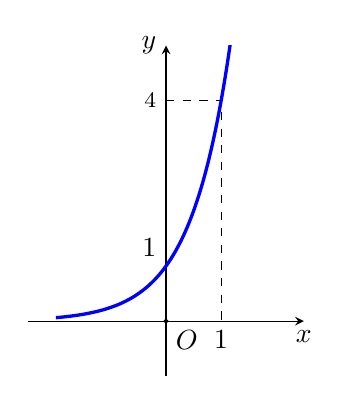
\begin{tikzpicture}[scale=0.7,>=stealth] 
	\draw[->] (-2.5,0) -- (2.5,0) node[below] {$x$}; 
	\draw[->] (0,-1) -- (0,5) node[left] {$y$}; 
	\draw[fill=black] (0,0) node[below right]{$O$} circle (1pt);
	\draw (0,1) node[above left]{$1$}; 
	\draw (1,0) node[below]{$1$}; 
	\draw (0,4) node[left]{\footnotesize$4$}; 
	\tkzDefPoints{1/4/A} 
	\tkzDrawPoints[fill=black](A) 
	\draw [dashed] (0,4)--(1,4)--(1,0); 
	\begin{scope}
		\clip (-2,-0.5) rectangle (2,5);
		\draw[color=blue,very thick,smooth,samples=200, domain=-2:2.01] plot (\x,{(4)^(\x)}); 
	\end{scope}
\end{tikzpicture} }
	\loigiai{ 
		a) Hàm số đã cho có tập giá trị là $\mathbb{R}$ là khẳng định sai. Hàm số đã cho có tập giá trị là $(0;+\infty)$.\\ 
		b) Hàm số không liên tục trên $\mathbb{R}$ là khẳng định sai.\\ 
		c) Dựa vào đồ thị ta có $\displaystyle a=4 \Rightarrow y=4^x$ nên đồ thị hàm số đi qua điểm ${(-1;\dfrac{1}{4})}$ là khẳng định đúng.\\ 
		d) Vì ${4}>1$ nên hàm số đã cho đồng biến trên $\mathbb{R}$.\\ 
		
}\end{ex}

\begin{ex}
	Cho đồ thị hàm số $y=f(x)=\log_a x$ với $a>0,a \ne 1$ có đồ thị như hình vẽ. Xét tính đúng sai của các khẳng định sau
	\begin{center}
		\begin{tikzpicture}[>=stealth] 
	\draw[->] (-1,0) -- (7.5,0) node[below] {$x$}; 
	\draw[->] (0,-1.5) -- (0,2.5) node[left] {$y$}; 
	\draw[fill=black] (0,0) node[below right]{$O$} circle (1pt);
	\draw (0,1) node[left]{$1$}; 
	\draw (1,0) node[below]{$1$}; 
	\draw (7,0) node[below]{$7$}; 
	\draw[fill=black] (7, 1) circle (1pt);
	\draw [dashed] (0,1)--(7,1)--(7,0); 
	\begin{scope}
		\clip (-1,-1.5) rectangle (7.5,2.5);
		\draw[color=blue,thick,smooth, samples = 200, domain=0.001:7.5] plot (\x,{(ln(\x)/ln(7)}); 
	\end{scope}
\end{tikzpicture}
	\end{center}
	\choiceTF
	{ \True Hàm số đã cho có tập xác định là $(0;+\infty)$ }
	{ \True Trên khoảng $(8;+\infty)$ thì hàm số đã cho đồng biến }
	{ \True Đồ thị hàm số đã cho đi qua điểm ${(\dfrac{1}{49};-2)}$ }
	{ $\lim\limits_{x\to 0^+}f(x)=0$}
	\loigiai{ 
		a) Hàm số đã cho có tập xác định là $(0;+\infty)$ là khẳng định đúng\\ 
		b) Dựa vào đồ thị ta có $\displaystyle a=7\Rightarrow y=\log_7 x$ nên đồ thị hàm số đi qua điểm ${(\dfrac{1}{49};-2)}$ là khẳng định đúng.\\ 
		c) Trên khoảng $(8;+\infty)$ thì hàm số đã cho đồng biến là khẳng định đúng.\\ 
		d) $\lim\limits_{x\to 0^+}f(x)=-\infty$.
}\end{ex}


\Closesolutionfile{ans}

\ind{PHẦN III.} \inden{Câu trắc nghiệm trả lời ngắn.}\\
\Opensolutionfile{ans}[ans/1D6-B3-3]

\begin{ex}%[2D2B4-3]
	Cho hai đồ thị $(C_1) \colon y=2^x$ và $(C_2) \colon y=3^{-x}$. Gọi $M$, $N$ lần lượt là hai điểm thuộc $(C_1)$ và $(C_2$). Biết $M$ và $N$ đối xứng nhau qua $I\left(0;\tfrac{5}{2} \right)$. Tính độ dài đoạn $MN$ (kết quả làm tròn đến hàng phần trăm). \\
	\shortans[oly]{$2{,}24$}
	\loigiai{
		Gọi $M\left(m;2^m \right) \in (C_1)$. Do $I$ là trung điểm của đoạn $MN$ nên $N\left( -m;5-2^m\right)$
		\begin{itemize}
			\item [$\bullet$] $N \in (C_2)$, suy ra $5-2^m=3^m \Leftrightarrow 3^m+2^m=5 \Leftrightarrow m=1$;
			\item [$\bullet$] Từ đây, tính được $M(1;2)$ và $N(-1;3)$.
		\end{itemize}
		Độ dài $MN=\sqrt{5} \approx2,24$.
	}
\end{ex}

\begin{ex}%[1D4K3-4]
	Cô Yên gửi $10$ triệu đồng vào ngân hàng theo hình thức lãi kép có kì hạn là $12$ tháng với lãi suất $6 \% /$năm. Giả sử qua các năm thì lãi suất không thay đồi và cô Yên không gửi thêm tiền vào mỗi năm. Để biết sau $y$ (năm) thì tổng số tiền cả vốn và lãi có được là $x$ (đồng), cô Yên sử dụng công thức $y=\log _{1{,}06}\left(\frac{x}{10}\right)$. Hỏi sau ít nhất bao nhiêu năm thì cô Yên có thể rút ra dược số tiền $15$ triệu đồng từ tài khoản tiết kiệm đó (làm tròn kết quả đến hàng đơn vị)?\\
	\shortans[oly]{$7$}
	\loigiai{
		Cô Yên có thể rút ra được số tiền 15 triệu đồng sau ít nhất số năm là
		$$
		y=\log _{1{,}06}\left(\frac{15}{10}\right) \approx 7 \text { (năm). }
		$$}
\end{ex}

\begin{ex}
	Số lượng của một loại vi khuẩn X trong phòng thí nghiệm được tính theo công thức $x(t)=x(0)\cdot 2^t$, trong đó $x(0)$ là số lượng vi khuẩn X ban đầu, $x(t)$ là số lượng vi khuẩn X sau $t$ (phút). Biết sau 2 phút thì số lượng vi khuẩn X là 625 nghìn con. Hỏi sau bao nhiêu phút, kể từ lúc bắt đầu, số lượng vi khuẩn X là 10 triệu con?\\
	\shortans[oly]{$6$}
	\loigiai{
		Ta có $x(2)=x(0)\cdot 2^2=625000\Rightarrow x(0)=156250$.\\
		Xét $x(t)=x(0)\cdot 2^t=10000000\Rightarrow 2^t=\dfrac{10000000}{156250}=64\Rightarrow t=6$.\\
		Vậy sau $6$ phút kể từ lúc bắt đầu thì số lượng vi khuẩn X là 10 triệu con.
	}
\end{ex}

\begin{ex}%[1D4K3-4]
	Các nhà tâm lí học sử dụng mô hình hàm số mũ để mô phỏng quá trình học tập của một học sinh như sau: $f(t)=c\left(1-\mathrm{e}^{-k}\right)$, trong đó $c$ là tổng số đơn vị kiến thức học sinh phải học, $k$ (kiến thức/ngày) là tốc độ tiếp thu của học sinh, $t$ (ngày) là thời gian học và $f(t)$ là số đơn vị kiến thức học sinh đã học được.
	\begin{flushright}
		\textit{(Nguồn: R.I. Charles et al., Algebra 2, Pearson).}
	\end{flushright}
	Giả sử một em học sinh phải tiếp thu $25$ đơn vị kiến thức mới. Biết rằng tốc độ tiếp thu của em học sinh là $k=0{,}2$. Hỏi em học sinh sẽ học được (khoảng) bao nhiêu đơn vị kiến thức mới sau $8$ ngày (Làm tròn kết quả đến hàng đơn vị)?\\
	\shortans[oly]{$20$}
	\loigiai{
		Sau $2$ ngày, em học sinh đó học được số đơn vị kiến thức mới là
		$$
		f(2)=25 \cdot\left(1-\mathrm{e}^{-0,2 \cdot 2}\right) \approx 8 \text { (đơn vị kiến thức). }
		$$
		Sau $8$ ngày, em học sinh đó học được số đơn vị kiến thức mới là
		$$
		f(8)=25 \cdot\left(1-\mathrm{e}^{-0,2 \cdot 8}\right) \approx 20 \text { (đơn vị kiến thức). }
		$$
	}
\end{ex}

\begin{ex}%[TEX SBT CTST, Thành Đức Trung]%[1D4K3-4]
	Sau khi bệnh nhân uống một liều thuốc, lượng thuốc còn lại trong cơ thể giảm dần và được tính theo công thức $D(t)=D_0\cdot a^t$ (mg), trong đó $D_0$ và $a$ là các hằng số dương, $t$ là thời gian tính bằng giờ kể từ thời điểm uống thuốc. Biết rằng bệnh nhân đã uống 100 mg thuốc và sau 1 giờ thì lượng thuốc trong cơ thể còn 80 mg. Hỏi sau 5 giờ, lượng thuốc đã giảm đi bao nhiêu phần trăm so với lượng thuốc ban đầu (kết quả làm tròn đến hàng phần chục)?\\
	\shortans[oly]{$67{,}2$}
	\loigiai
	{Theo bài ra $D_0=100$ mặt khác $D(1)=80$ nên $D_0\cdot a^1=80\Leftrightarrow 100\cdot a=80\Leftrightarrow a=0{,}8$.\\
		Sau 5 giờ, lượng thuốc trong cơ thể là 
		\[D(5)=D_0\cdot a^5=D_0\cdot 0{,}8^5=32{,}768\%\cdot D_0.\]
		Vậy sau 5 giờ lượng thuốc đã giảm đi $100\%-32{,}768\%=67{,}2\%$ so với lượng thuốc ban đầu. 
	}
\end{ex}
\Closesolutionfile{ans}

